%% One compromised node, how many stores?
%% One-column layout based on the CEUR-WS class (ceurart).
%% Build: latexmk -pdf main.tex
%% arXiv source bundle: python ../make_arxiv.py
\documentclass{ceurart}

\sloppy
\graphicspath{{../../figures/en/}}

\newcommand{\degC}{\,\textdegree{}C}

\begin{document}

\copyrightyear{2026}
\copyrightclause{Copyright for this paper by its author.
  Use permitted under Creative Commons License Attribution 4.0 International (CC BY 4.0).}

\conference{Preprint, November 2026}

\title{One Compromised Node, How Many Stores? Blast Radius and In-Store Defences in Supermarket Refrigeration Remote Management}

\author[1]{Fabio Greco}
\fnmark[1]
\address[1]{Independent researcher, Naples, Italy}
\fntext[1]{MSc student in Computer Engineering at the University of Naples Federico II. This work was carried out independently and is not affiliated with the University.}

\begin{abstract}
In October and November 2026 the refrigeration controllers of supermarkets in several European countries, including about 700 sites in France and stores in Italy, were remotely manipulated to force prolonged high-temperature defrost cycles.
This paper asks how many stores a single compromised remote-management node can affect, and which in-store defences limit the damage even when that node is controlled by the attacker.
We combine a lumped first-order thermal model of a freezer cabinet in state-space form, a hypothetical chain of 20 stores in Campania, three remote-management architectures and a scripted attacker that anticipates a defrost duration limit.
In the worst case, one compromised node reaches 20, 8 or 1 store depending on the architecture.
A local command filter with a maximum defrost duration and a minimum interval between defrosts reduces the time above the $-15$\degC{} threshold from at least 352 to 53 minutes, within the 60-minute loss criterion of the study, provided that the interval prevents another remote defrost before staff take over.
An independent alarm meets the criterion only with a response within about 15 minutes, which may be difficult to guarantee at night without an automatic response.
Closed-form solutions reproduce the simulation and give the maximum admissible defrost duration, about 33 minutes for the base cabinet; varying the cabinet's thermal parameters shows that such limits must be computed for each cabinet.
A break-even condition gives the yearly attack probability above which an in-store protection pays for itself.
Reducing the blast radius and enforcing limits inside each store are complementary.
Parameters are illustrative: the results describe a mechanism, not measurements of real installations.
\end{abstract}

\begin{keywords}
  cyber-physical systems security \sep
  remote management \sep
  commercial refrigeration \sep
  blast radius \sep
  defence in depth \sep
  simulation
\end{keywords}

\maketitle

%% ===========================================================================
\section{Introduction}

In retail, refrigerated cabinets and cold rooms are regulated by electronic controllers connected to remote supervision systems.
Supervision is often outsourced to installers and maintenance companies, which follow many stores from a single workstation.
This reduces operating costs, but it also creates a channel through which a single command can change the behaviour of many installations at once.

The events of October and November 2026, summarised in Section~\ref{sec:background}, showed that this channel can be exploited.
Defrost cycles were forced at night, with the stores closed, and by morning the goods had to be discarded.
Public discussion focused on who the attackers were and how they gained access.
This paper addresses a complementary, architectural question: once a node is compromised, how much damage can it do, and what limits it?

The starting point is an analogy from software engineering: the \emph{single point of failure}, a component whose failure stops the whole system.
A centralised remote-management node is a single point of failure for availability, but the 2026 attacks exposed a different property: the node keeps working and issues harmful commands.
We therefore treat it as a single point of \emph{compromise}, a failure of integrity rather than of availability.
We study it with tools from systems theory, a state-space model of the cabinet with closed-form solutions, and from engineering economics, a break-even analysis of the countermeasures.

We pose two research questions:
\begin{description}
  \item[RQ1] How many stores does a compromised remote-management node affect, as the remote-management architecture varies?
  \item[RQ2] Which defences placed inside the store limit the damage even when the node is compromised, and with what margins?
\end{description}

The contributions are four:
\begin{enumerate}
  \item an operational definition of the \emph{blast radius} of a node, and a comparison of three architectures on a hypothetical chain of 20 stores in Campania;
  \item a minimal, reproducible thermal model of a forced defrost in a freezer cabinet, written in state-space form, with closed-form expressions for the time above the threshold, the maximum admissible defrost duration and the maximum alarm response time;
  \item a simulation-based evaluation of a local command filter, of an independent alarm and of an automatic protection against a scripted attacker that anticipates a duration limit, with a sensitivity analysis that includes the cabinet's thermal parameters;
  \item a set of practical countermeasures tied to the results, including a non-networked temperature band limiter and a break-even condition for its cost, together with open code to reproduce them.
\end{enumerate}

Section~\ref{sec:background} summarises the known facts and related work.
Section~\ref{sec:problem} defines the problem and the threat model, Section~\ref{sec:method} the model and the method.
Sections~\ref{sec:results}, \ref{sec:countermeasures} and~\ref{sec:limitations} present results, countermeasures and limitations; Section~\ref{sec:conclusions} concludes.

%% ===========================================================================
\section{Background and related work}
\label{sec:background}

\subsection{The October--November 2026 attacks}

The following facts are reconstructed from official and press sources and are current as of 18 November 2026.
Table~\ref{tab:timeline} summarises the timeline.

\begin{table}[ht]
  \caption{Essential timeline of the events.}
  \label{tab:timeline}
  \begin{tabular}{@{}p{0.13\linewidth}p{0.67\linewidth}p{0.12\linewidth}@{}}
    \toprule
    Date & Event & Ref. \\
    \midrule
    11--12 Oct & France: refrigeration controllers of about 700 sites compromised in one night; defrost settings changed to high temperatures; at least 15 fires & \cite{anssi2026attribution,certfr2026cti009} \\
    13 Oct & Italy: the National Cybersecurity Agency (ACN) publishes urgent verification and mitigation measures for food retail and the cold chain & \cite{cyber360acn2026} \\
    2 Nov & Second wave in nine countries: Belgium, Estonia, Finland, Ireland, Italy, Luxembourg, the Netherlands, Portugal and Sweden; more than 115 stores in six of them & \cite{euronews2026nine,bleeping2026wave} \\
    Early Nov & Italy: cases in more than ten regions, including at least four supermarkets in Sicily, collective catering and food logistics & \cite{euronews2026nine,cyber360cases2026} \\
    3 Nov & ACN draws renewed attention to its bulletin, asking for six immediate checks: internet exposure, OT networks, maintenance providers, credentials, temperatures, unsupported devices & \cite{cyber360acn2026} \\
    9--10 Nov & France attributes the October campaign to Shahid Kaveh, an offensive cyber unit linked to Iran's Islamic Revolutionary Guard Corps & \cite{anssi2026attribution,mfa2026attribution} \\
    10 Nov & Three supermarkets in Naples and two in its province reported as hit on 1--2 November (single source) & \cite{fanpage2026napoli} \\
    \bottomrule
  \end{tabular}
\end{table}

In France the retailers involved included at least 300 Intermarch\'e and Netto stores, 80 Carrefour and about thirty Monoprix, as well as Coop\'erative U and E.Leclerc stores~\cite{open2026francia}.
The French government estimates the spoiled goods at tens of millions of euros~\cite{mfa2026attribution}.
In Italy the reported cases are mostly defrost or temperature manipulations; one report describes a defrost extended beyond 250 minutes and another a setpoint raised to 150\degC~\cite{cyber360cases2026}.

Public information on how access was obtained is partial.
Press reports indicate that older versions of the controllers' regulation software were targeted~\cite{fatto2026francia}, and the manufacturer considers that outdated or non-updated equipment was involved~\cite{lmi2026danfoss}.
The French attribution statement refers technical details to separate CERT-FR documents~\cite{anssi2026attribution,certfr2026cti009}.
Two paths emerge from the sources:
\begin{itemize}
  \item \textbf{Through a shared system.} In Sweden all the affected stores of one chain were connected to the same external refrigeration control system, and in Portugal the attack appears to have targeted an external company managing refrigeration~\cite{thn2026wave}.
  \item \textbf{Directly on each store.} In the Belgian cases the attackers reportedly entered the systems of individual supermarkets, not those of refrigeration contractors~\cite{thn2026wave}.
\end{itemize}
Industry experts note that many installations are remotely managed, often by third parties, and do not receive the necessary software updates~\cite{aljazeera2026coldwar}.

Two pro-Russian groups claimed the attacks, including those in Italy, but the claims are unverified~\cite{punto2026claims}.
The French attribution concerns the October campaign in France and does not automatically extend to the 2 November wave.
Attribution is not relevant to this work, which studies the architectural consequences of remote access once obtained.
For Campania only one press report is available~\cite{fanpage2026napoli}, and the cases it describes do not appear in a national overview of Italian incidents~\cite{cyber360cases2026}.
There is no public information on how centralised remote management of supermarkets in the region is; for this reason the store chain studied below is hypothetical.

\subsection{Related work}

\paragraph{Security of remotely managed cyber-physical systems.}
Attacks on industrial control systems have repeatedly shown that control channels can be turned into physical damage, from Stuxnet~\cite{langner2011stuxnet} to the 2015 attack on the Ukrainian power grid, where the attackers, working remotely, used the operators' own control interfaces to open breakers in substations of three distribution companies~\cite{lee2016ukraine}; surveys of cyber-physical systems security classify such attacks and the corresponding defences~\cite{humayed2017cps}.
C\'ardenas et al.\ showed how physical models of the controlled process can be used to assess the impact of attacks and to detect and respond to them~\cite{cardenas2011attacks}, and a large body of work on physics-based attack detection followed~\cite{giraldo2018survey}.
Third-party remote access is a recurring entry point: in the 2013 Target breach the attackers reportedly first gained access with credentials stolen from an HVAC and refrigeration contractor that had remote access to the retailer's network~\cite{senate2014target}.
Refrigeration controllers have also been studied directly: in 2025 Armis reported ten vulnerabilities in Copeland E2 and E3 controllers, which manage refrigeration, HVAC and lighting, that combined could allow unauthenticated remote code execution~\cite{armis2025frostbyte}.
Operational technology guidance recommends network segmentation and defence in depth~\cite{nist80082r3}.
This work does not address detection or intrusion; it quantifies how far one compromised node reaches and how much damage limits placed in each store can prevent.

\paragraph{Thermal models of commercial refrigeration.}
Control studies of supermarket refrigeration describe cold rooms and display cases with lumped energy balances; the benchmark of Hovgaard et al., for example, uses a single energy balance for the cold-room temperature and refers to hysteresis control as the common practice~\cite{hovgaard2011benchmark}.
Measurements under test conditions show that the temperature inside a cabinet varies with position, the warmest readings being in the areas most exposed to ambient air~\cite{evans2007cabinets}.
We use the same kind of lumped model, but for a different purpose: to compute the effect of a forced defrost and the design limits of the defences, keeping in mind that a single temperature is only a proxy for a spatially varying one.

\paragraph{Independent protection layers.}
In the process industry, safety functions are implemented in safety instrumented systems kept separate from the basic process control system~\cite{iec61511}.
The TRITON attack, in which the attackers reprogrammed the safety controllers of a petrochemical plant, showed that such systems can themselves be targeted when they are reachable from the network~\cite{dipinto2018triton}.
The temperature band limiter discussed in Section~\ref{sec:method} applies the same principle at a much smaller scale: a separate, non-networked device that bounds the physical outcome whatever commands arrive.

\paragraph{Economics of security investment.}
Gordon and Loeb modelled how much to invest in protecting an information set as a function of its vulnerability and of the potential loss, showing that for two broad classes of breach-probability functions the optimal investment does not exceed about 37\% of the expected loss~\cite{gordon2002economics}.
Anderson and Moore observed that systems are particularly prone to failure when the party guarding them is not the party that suffers when they fail~\cite{anderson2006economics}, which is the situation of a retailer whose refrigeration is remotely managed by a maintenance company.
The break-even condition used in Section~\ref{sec:countermeasures} is the elementary special case of a protection that removes the loss it targets; it is not a new economic model.

The individual tools used here, a state-space model, its exponential solution and a break-even condition, are standard.
The contribution of this work lies in combining them into a quantitative assessment of how far a single compromise reaches, what in-store limits can still prevent, and when such limits are worth their cost.

%% ===========================================================================
\section{Problem and threat model}
\label{sec:problem}

\subsection{Blast radius}

We call \emph{remote-management node} any point from which commands can be sent to the installations: a supervisor, a gateway, a maintenance company's account.
The \emph{blast radius} of a node is the number of stores that node can command.
If several stores depend on the same node, its compromise is a common-cause failure: a single event affects all of them together.
The node is a shared critical dependency, analogous to a single point of failure in software engineering; in the scenario considered here, however, its compromise makes it a single point of compromise: the node remains operational but loses integrity and issues unauthorised commands.
For an architecture with $n$ nodes, where node $i$ reaches $s_i$ stores, the worst-case and average blast radius are
\begin{equation}
  B_{\max} = \max_{i} s_i, \qquad B_{\mathrm{avg}} = \frac{1}{n}\sum_{i=1}^{n} s_i,
\end{equation}
the average assuming that every node is equally likely to be compromised.

\subsection{Threat model}

The attacker controls \emph{one} node and can send defrost commands to every store that node reaches.
This matches the French authorities' description of the October campaign, in which defrost settings were changed to high temperatures~\cite{anssi2026attribution}.
The attacker acts at 02:00, with the stores closed, using a \emph{script}: it knows the duration limit that a filter might impose, but receives no feedback on which commands are accepted.

The attacker has no physical access to the stores and cannot modify the defences installed in them.
How the node is compromised is outside the scope of this work, which does not describe intrusion techniques.

\subsection{Store chain and architectures}

We consider a hypothetical chain of 20 stores in Campania: 8 in the province of Naples, 5 in Salerno, 4 in Caserta, 2 in Avellino and 1 in Benevento.
Remote management can be organised in three ways (Table~\ref{tab:architectures}, Figure~\ref{fig:architectures}).

\begin{table}[ht]
  \caption{The three remote-management architectures compared.}
  \label{tab:architectures}
  \begin{tabular}{@{}lrl@{}}
    \toprule
    Architecture & Nodes & Stores reached by each node \\
    \midrule
    A. Centralised & 1 & 20 \\
    B. One node per province & 5 & 8, 5, 4, 2, 1 \\
    C. One node per store & 20 & 1 \\
    \bottomrule
  \end{tabular}
\end{table}

\begin{figure}[ht]
  \centering
  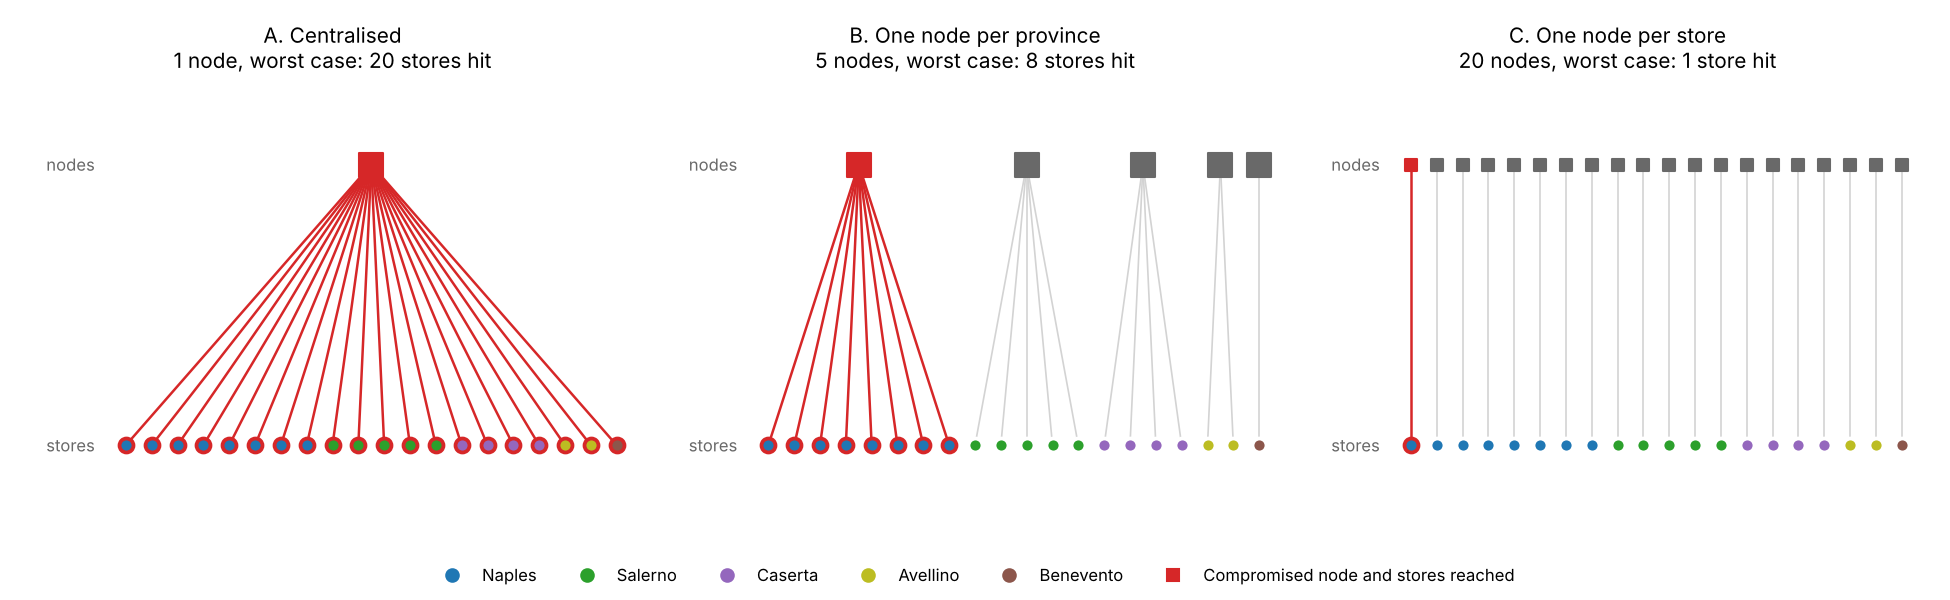
\includegraphics[width=\linewidth]{architectures.png}
  \caption{The three architectures. In red, the node compromised in the worst case and the stores it reaches. Store colours indicate the province.}
  \label{fig:architectures}
\end{figure}

Architecture C does not remove the risk.
If every store shares the same exposed weakness, the attacker can hit them one by one, as seems to have happened in Belgium~\cite{thn2026wave}.
This is why we also evaluate defences that do not depend on the architecture.

%% ===========================================================================
\section{Model and method}
\label{sec:method}

\subsection{Thermal model of the cabinet}

The freezer cabinet is represented by a single temperature $T$: the mean temperature of the cabinet and its contents, with structure, air and products lumped together.
$T$ changes because of three terms: heat entering from the store, proportional to the temperature difference; heat removed by the compressor when it is on; heat added by the defrost heaters when they are on:
\begin{equation}
  C \frac{dT}{dt} = UA\,(T_{amb} - T) - P_f\,u_c(t) + P_s\,u_s(t),
  \label{eq:model}
\end{equation}
where $u_c$ and $u_s$ are 1 when the compressor and the heaters are on, and 0 otherwise.
In normal operation a hysteresis thermostat switches the compressor on above $-17$\degC{} and off below $-19$\degC.
During a defrost the compressor is off and the heaters are on.
$P_f$ and $P_s$ are the effective thermal powers removed from and added to the lumped mass in the model, not necessarily the nominal electrical ratings of the compressor and of the heaters.

In the input-state-output (state-space) form used in systems theory, the state is $x = T$, the inputs are $u_c$ and $u_s$, the store temperature $w = T_{amb}$ is a disturbance and the output is $y = x$:
\begin{equation}
  \dot{x} = -\frac{1}{\tau}\,(x - w) - \frac{P_f}{C}\,u_c + \frac{P_s}{C}\,u_s, \qquad y = x, \qquad \tau = \frac{C}{UA}.
  \label{eq:ss}
\end{equation}
In the usual notation $\dot{x} = Ax + Bu + Ew$ with $u = [u_c, u_s]^\top$, this means $A = -1/\tau$, $B = [-P_f/C,\ P_s/C]$ and $E = 1/\tau$.
The system is linear, time-invariant and of first order, with the single eigenvalue $-1/\tau$; it is therefore asymptotically stable.
The thermostat closes a feedback loop with hysteresis on $u_c$, so the closed loop is a switched system: between two switches the inputs are constant and the state relaxes exponentially towards the equilibrium $x_{eq} = T_{amb} + (P_s u_s - P_f u_c)/UA$.
Equation~\eqref{eq:model} is integrated with the explicit Euler method and a step of $\Delta t = 10$\,s:
\begin{equation}
  T_{k+1} = T_k + \frac{\Delta t}{C}\left[ UA\,(T_{amb} - T_k) - P_f\,u_{c,k} + P_s\,u_{s,k} \right].
\end{equation}
Table~\ref{tab:parameters} lists the parameters.

\begin{table}[ht]
  \caption{Model parameters (illustrative).}
  \label{tab:parameters}
  \begin{tabular}{@{}lr@{}}
    \toprule
    Parameter & Value \\
    \midrule
    Store temperature $T_{amb}$ & 22\degC \\
    Setpoint and hysteresis & $-18 \pm 1$\degC \\
    Threshold & $-15$\degC \\
    Thermal conductance $UA$ & 20\,W/\textdegree{}C \\
    Heat capacity $C$ & 300{,}000\,J/\textdegree{}C \\
    Cooling power $P_f$ & 1{,}600\,W \\
    Defrost power $P_s$ & 600\,W \\
    Integration step $\Delta t$ & 10\,s \\
    \bottomrule
  \end{tabular}
\end{table}

The heat capacity $C$ is an illustrative composition: for example 120\,kg of frozen products with a specific heat of about 2\,kJ/(kg\,K), i.e.\ 240\,kJ/\textdegree{}C, plus about 60\,kJ/\textdegree{}C for the structure, shelves and evaporator; the air of a 0.5\,m$^3$ cabinet alone would contribute about 0.6\,kJ/\textdegree{}C.
The linear model neglects the latent heat of melting, which becomes significant as the products approach their initial freezing point, a few degrees below 0\degC.
The decisive scenarios peak at $-9.3$ and $-12.3$\degC{} (Section~\ref{sec:results}), where this effect is smaller; the scenarios that go above 0\degC{} exceed the loss criterion before reaching 0\degC, so their classification does not depend on it.

The time constant $\tau = C/UA$ is 250 minutes.
The equilibria are $T_s = 22 + 600/20 = 52$\degC{} under continuous defrost, an asymptotic value reached only under a prolonged continuous defrost (after 300 minutes the model gives 31.2\degC), of the same order as the roughly 50\degC{} reported in the press~\cite{fatto2026francia}, which is not a calibration; $T_c = 22 - 1600/20 = -58$\degC{} with the compressor always on, so the cooling margin is ample; and 22\degC{} with everything off.

\subsection{Closed-form results}

With constant inputs, the solution of Equation~\eqref{eq:ss} is the sum of the free and the forced response:
\begin{equation}
  x(t) = x_{eq} + (x_0 - x_{eq})\,e^{-t/\tau}.
\end{equation}
Starting from the cabinet temperature at 02:00 (about $-17$\degC), after 300 minutes of defrost this gives 31.2\degC, the same value as the simulation.
For a defrost of duration $d$ starting from $T_0$, the same solution gives, without simulation, the time to cross the threshold $T_{th} = -15$\degC, the peak temperature, the recovery time with the compressor on and the minutes above the threshold:
\begin{align}
  t_1 &= \tau \ln\frac{T_s - T_0}{T_s - T_{th}}, &
  T_p(d) &= T_s + (T_0 - T_s)\,e^{-d/\tau}, \\
  t_r(d) &= \tau \ln\frac{T_p(d) - T_c}{T_{th} - T_c}, &
  M(d) &= d - t_1 + t_r(d) \quad (d > t_1).
\end{align}
The recovery formula holds because the thermostat keeps the compressor on as long as $x > -17$\degC.
The \emph{maximum admissible defrost duration} $d_{\max}$ is the solution of $M(d) = 60$ minutes.
With an alarm that fires 10 minutes after the threshold is crossed and a response time $r$, the defrost lasts $t_1 + 10 + r$, so the \emph{maximum response time} is $r_{\max} = d_{\max} - t_1 - 10$.
These expressions verify the code against the model and turn the simulation results into design limits; they are not a validation of the model against real cabinets.

\subsection{Threshold and loss criterion}

The threshold of $-15$\degC{} is $-18$\degC{} plus the maximum tolerance of 3\degC{} allowed for quick-frozen foods in retail display cabinets by Directive 89/108/EEC~\cite{eu1989frozen}, transposed in Italy by Legislative Decree 110/1992, Article~4~\cite{dlgs1101992}.
The directive refers to the temperature of the product; here it is applied to the lumped temperature $T$ as a proxy.
We say that a store \emph{exceeds the loss criterion} if its cabinet stays above $-15$\degC{} for more than 60 cumulative minutes.
The 60 minutes are a convention of this study, not a regulatory limit, and exceeding the criterion is an indicator of thermal risk, not a food-safety or regulatory judgement.
For the economic estimate we assume goods worth \texteuro{}30{,}000 per store; the loss scales linearly with this value, which is consistent with the order of magnitude implied by the French estimate of tens of millions of euros over about 700 sites~\cite{anssi2026attribution,mfa2026attribution}.

\subsection{Scenario and attacker}

Each simulation covers one night, from 20:00 to 08:00.
The attack starts at 02:00.
At 07:00 staff arrive and switch the cabinet to local mode: any remote defrost in progress is interrupted, control returns to the thermostat, and from then on remote commands are ignored.
The attacker's script sends 13 commands: at 02:00 a 600-minute defrost and, also starting at 02:00 and then every 30 minutes until 07:30, the longest defrost a filter would allow (30 minutes).
With R1 alone, for example, the 600-minute command is rejected and the ten 30-minute commands from 02:00 to 06:30 are executed back to back, 300 minutes in total; those of 07:00 and 07:30 are ignored because the cabinet is then in local mode.
Overlapping commands have no additional effect, so we report the minutes of defrost actually executed rather than the number of commands.
The switch to local mode at 07:00 takes precedence over any remote command arriving at the same instant.

\subsection{Defences}

All defences are placed inside the store, downstream of the compromised node; on the node itself the attacker could disable them.
\begin{itemize}
  \item \textbf{Local command filter.} Checks every defrost command against two rules: R1, a maximum duration of 30 minutes; R2, at least 6 hours between the start times of two accepted defrosts.
  \item \textbf{Independent alarm with technician.} A sensor separate from the control system fires after 10 consecutive minutes above the threshold. A technician arrives 60 minutes later and switches the cabinet to local mode.
  \item \textbf{Automatic protection (temperature band limiter).} The same independent sensor, but the device itself stops the defrost as soon as it fires, without waiting for a person. It is the simplest case of a limiter that does not let the temperature stay outside a band $[T_{\min}, T_{\max}]$ for longer than a set time, acting on the actuators rather than on the commands.
\end{itemize}
In practice these defences rely on three properties: the limits are enforced by a device separate from the supervised controller, for example a safety relay in series with the defrost heater circuit; their settings can be changed only locally, not through the remote-management channel; and they use their own temperature sensor and keep a local event log.
Whether existing controllers can provide these properties is outside the scope of this paper.

The independent sensor measures a local temperature, for example that of a probe placed in a product simulant, not the lumped temperature $T$ of the model.
In the simulation we assume that the two coincide; on a real cabinet the relation between the measured temperature and the state of the goods, and therefore the alarm threshold, would have to be calibrated (Section~\ref{sec:limitations}).

The band limiter is meant to keep the goods within the criterion: its upper bound sits near $-15$\degC, as in scenario 4.
A lower bound could protect against an attacker driving the cabinet too cold, which wastes energy and stresses the compressor, through a protective action on the compressor itself.
Protecting the equipment from dangerous overheating, which matters given the fires reported in France~\cite{anssi2026attribution}, is a different function: it needs sensors placed at the relevant points, such as heaters and electrical connections, and limits set by the manufacturer, which a sensor of the cabinet's mean temperature cannot provide.
Being hardware and not networked, the limiter cannot be reconfigured remotely, but it has its own failure modes: sensor faults, spurious trips and physical tampering.
Its safe state on a fault concerns the function it protects: it removes power from the defrost heaters, while the compressor remains under the cabinet's local control logic rather than being forced on.

\subsection{Metrics}

For each scenario we measure the minutes of defrost executed, the peak temperature and the minutes above the threshold within the simulated window, until 08:00.
When the cabinet is still above the threshold at 08:00, the minutes above the threshold are a lower bound.

The sensitivity analysis varies one parameter at a time: the time from alarm to response (0--60 minutes), the maximum duration allowed by R1 (10--60 minutes), the minimum interval R2 (1--8 hours), the heat capacity $C$ (0.5 to 2 times its base value), the thermal conductance $UA$ (0.5 to 1.5 times), the defrost power $P_s$ (0.5 to 2 times) and the attack start time (02:00 to 02:25 in 5-minute steps, covering about one thermostat cycle).
We stop $UA$ at 1.5 times its base value because at twice the value the compressor, always on, would only bring the cabinet to $22 - 1600/40 = -18$\degC: it could never reach the $-19$\degC{} at which the thermostat switches it off, and the cabinet would be undersized even without an attack.
When a parameter changes, the temperature at 02:00 is recomputed from the normal night, because it depends on the thermostat phase.

%% ===========================================================================
\section{Results}
\label{sec:results}

\subsection{One cabinet under attack}

Without defences the cabinet exceeds the $-15$\degC{} threshold 8 minutes after the attack starts.
At 07:00, when staff arrive, it is at 31.2\degC, and at 08:00 it is still at 12.1\degC{} (Figure~\ref{fig:cabinet}).
Every store reached by the attacker therefore exceeds the loss criterion.

\begin{figure}[ht]
  \centering
  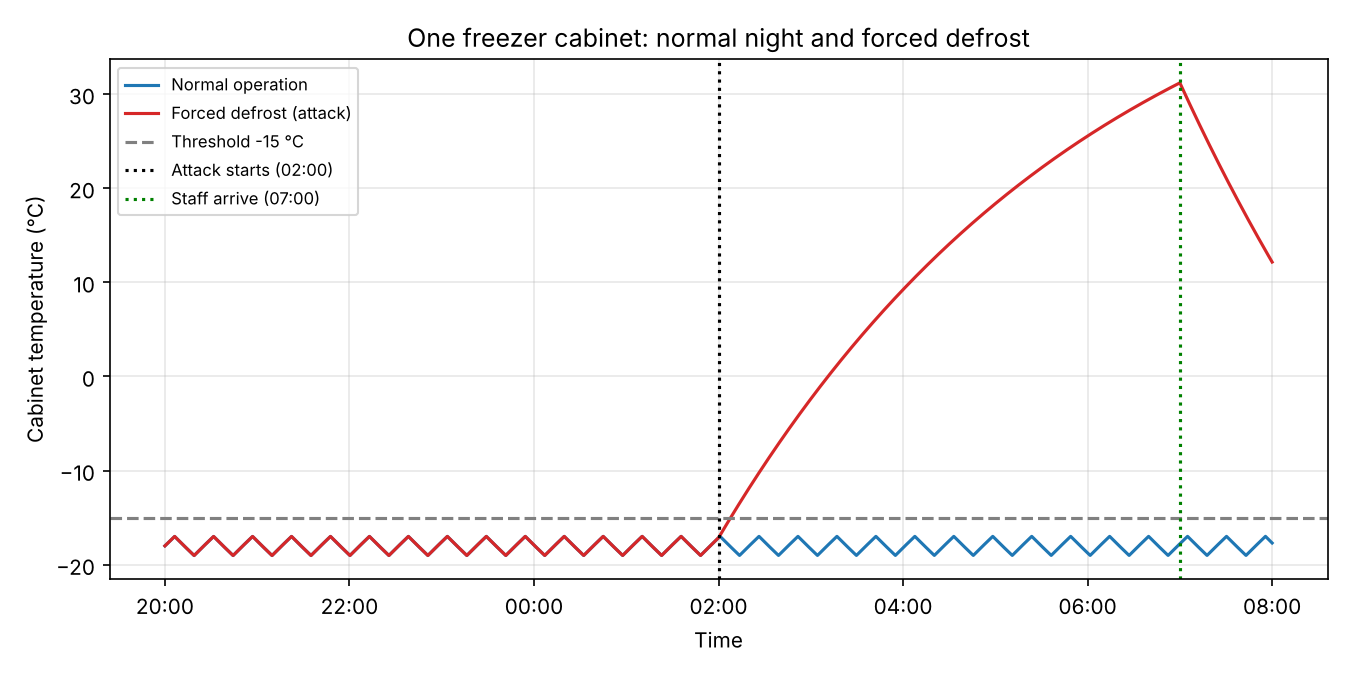
\includegraphics[width=0.85\linewidth]{cabinet.png}
  \caption{Temperature of a freezer cabinet during a normal night and with a forced defrost from 02:00 until staff arrive at 07:00.}
  \label{fig:cabinet}
\end{figure}

\subsection{Blast radius by architecture (RQ1)}

Table~\ref{tab:blast} reports the stores hit and the loss for each architecture, without in-store defences.

\begin{table}[ht]
  \caption{Stores hit and estimated loss with one compromised node, without in-store defences.}
  \label{tab:blast}
  \begin{tabular}{@{}lrrrr@{}}
    \toprule
    & \multicolumn{2}{c}{Stores hit} & \multicolumn{2}{c}{Loss (\texteuro)} \\
    \cmidrule(lr){2-3}\cmidrule(l){4-5}
    Architecture & worst & average & worst & average \\
    \midrule
    A. Centralised & 20 & 20 & 600{,}000 & 600{,}000 \\
    B. One node per province & 8 & 4 & 240{,}000 & 120{,}000 \\
    C. One node per store & 1 & 1 & 30{,}000 & 30{,}000 \\
    \bottomrule
  \end{tabular}
\end{table}

Compared with the centralised architecture, one node per province reduces the loss by 60\% in the worst case and by 80\% in the average case; one node per store reduces it by 95\%.
The worst case is the most relevant, because an attacker has an interest in targeting precisely the largest node (Figure~\ref{fig:loss}).

\begin{figure}[ht]
  \centering
  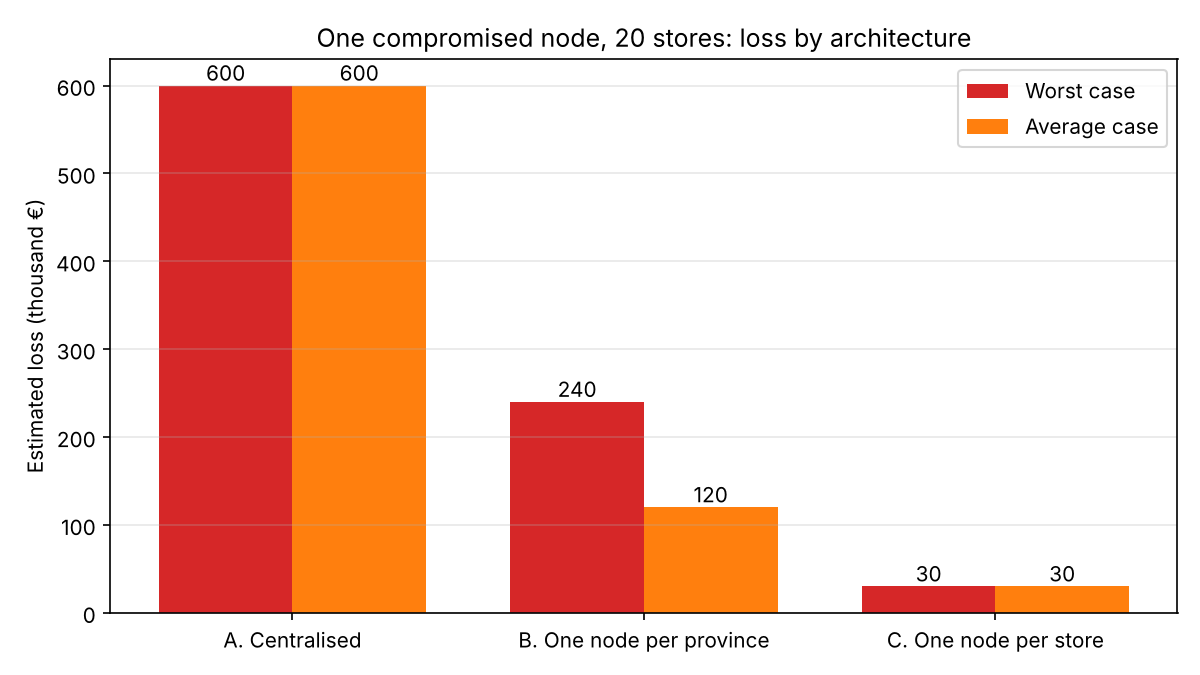
\includegraphics[width=0.75\linewidth]{loss.png}
  \caption{Estimated loss with one compromised node, by architecture.}
  \label{fig:loss}
\end{figure}

\subsection{In-store defences (RQ2)}

Table~\ref{tab:defences} compares five scenarios under the same attack.
The defences are installed in every store, so the results apply to each store reached, whatever the architecture.
The loss column uses the centralised architecture, where all 20 stores are reached: scenarios 2 and 4 therefore correspond to a centralised architecture with mandatory in-store limits.

\begin{table}[ht]
  \caption{Same attack, different defences. Loss computed on the centralised architecture (20 stores). In scenarios 0 and 1 the cabinet is still above the threshold at 08:00, so the minutes above the threshold are a lower bound.}
  \label{tab:defences}
  \begin{tabular}{@{}lrrrlr@{}}
    \toprule
    Scenario & \makecell[r]{Defrost\\executed (min)} & \makecell[r]{Peak\\temperature} & \makecell[r]{Minutes\\above threshold} & \makecell[l]{Loss\\criterion} & Loss (\texteuro) \\
    \midrule
    0. No defence & 300 & 31.2\degC & $\geq$352 & exceeded & 600{,}000 \\
    1. Filter, R1 only & 300 & 31.2\degC & $\geq$352 & exceeded & 600{,}000 \\
    2. Filter, R1 and R2 & 30 & $-9.3$\degC & 53 & met & 0 \\
    3. Alarm with technician & 78 & 1.4\degC & 151 & exceeded & 600{,}000 \\
    4. Automatic protection & 18 & $-12.3$\degC & 25 & met & 0 \\
    \bottomrule
  \end{tabular}
\end{table}

Four results emerge.

\paragraph{One rule is not enough.}
R1 rejects only the 600-minute command.
The 30-minute defrosts that follow are back to back and, until staff arrive at 07:00, have the same effect as a continuous defrost.

\paragraph{The two rules together keep the cabinet within the criterion.}
R2 accepts only the defrost at 02:00, because the next one would be allowed only at 08:00, after staff have switched the cabinet to local mode.
During the 30 minutes of defrost the cabinet rises to $-9.3$\degC, and the compressor needs about 30 more minutes to bring it back below the threshold: 53 minutes in total.
In the centralised architecture all 20 stores receive the command, but none exceeds the criterion.

\paragraph{An alarm that calls a technician is not enough.}
It fires at about 02:18 and the technician arrives at about 03:18, after 78 minutes of defrost.
The peak drops from 31.2 to 1.4\degC, but the cabinet stays above the threshold for 151 minutes.

\paragraph{An automatic protection is.}
With the same sensor stopping the defrost by itself, the defrost lasts 18 minutes, the peak is $-12.3$\degC{} and the cabinet stays above the threshold for 25 minutes (Figure~\ref{fig:defences}).

\begin{figure}[ht]
  \centering
  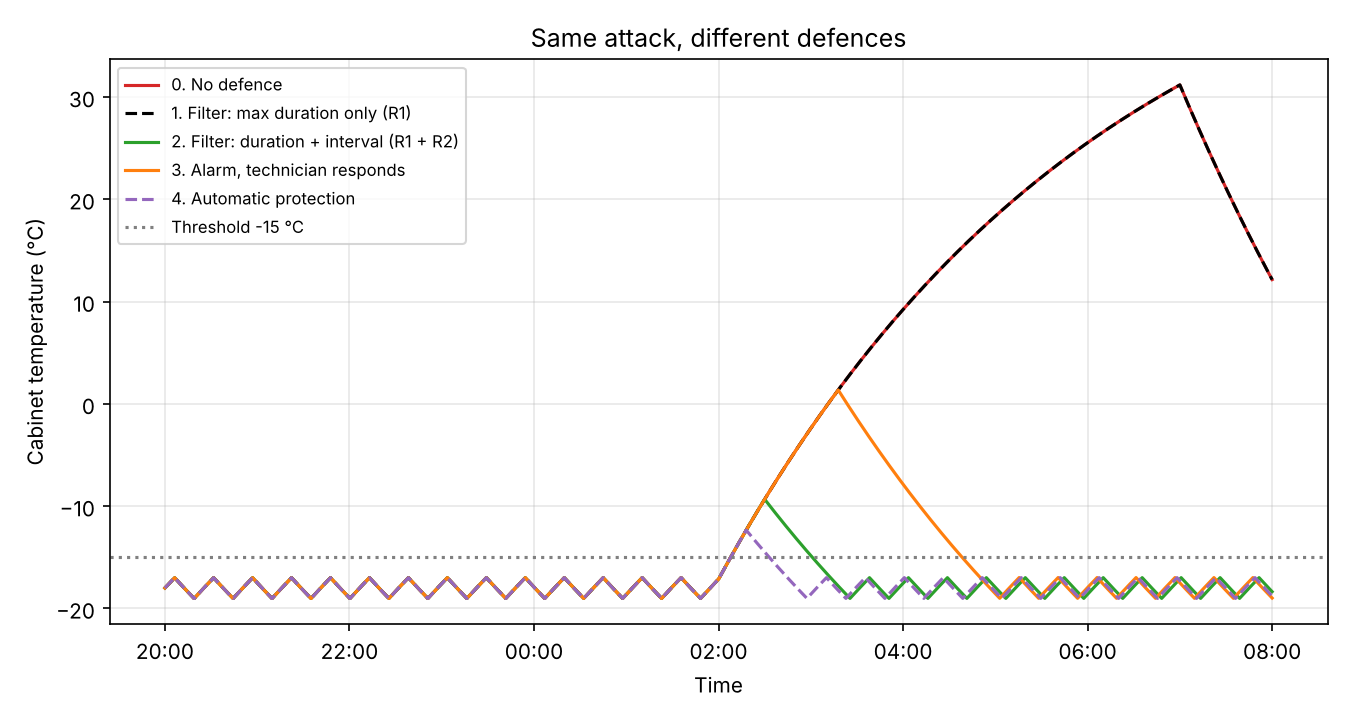
\includegraphics[width=0.85\linewidth]{defences.png}
  \caption{Cabinet temperature in the five defence scenarios. Scenarios 0 and 1 overlap.}
  \label{fig:defences}
\end{figure}

\subsection{Sensitivity analysis}

The margin of scenario 2, 53 minutes against a 60-minute criterion, is small.
Table~\ref{tab:sensitivity} and Figure~\ref{fig:sensitivity} show how the results change when one parameter is varied at a time.

\begin{table}[ht]
  \caption{Sensitivity to the parameters of the defences, of the cabinet and of the attack. Minutes above the threshold in brackets.}
  \label{tab:sensitivity}
  \begin{tabular}{@{}p{0.31\linewidth}p{0.15\linewidth}p{0.46\linewidth}@{}}
    \toprule
    Parameter varied & Range & Outcome \\
    \midrule
    Time from alarm to response (alarm) & 0--60 min & Criterion met up to 15 min (59), exceeded from 20 min (70); 0 min is scenario 4 (25) \\
    Maximum duration R1 (R1 and R2) & 10--60 min & Criterion met up to 30 min (53), exceeded from 35 min (64) \\
    Minimum interval R2 (R1 and R2) & 1--8 h & Criterion met from 4.75 h (53), exceeded at 4.5 h or less (94--322) \\
    Heat capacity $C$ & 0.5--2$\times$ & Filter: always met (31--56). Alarm with technician: always exceeded (134--162). Automatic protection: always met (24--26) \\
    Thermal conductance $UA$ & 0.5--1.5$\times$ & Filter: met up to 1$\times$ (20--53), exceeded from 1.25$\times$ (66--78). Alarm with technician: always exceeded (119--201). Automatic protection: always met (18--41) \\
    Defrost power $P_s$ & 0.5--2$\times$ & Filter: met up to 1$\times$ (42--53), exceeded from 1.5$\times$ (63--72). Alarm with technician: always exceeded (135--179). Automatic protection: always met (22--31) \\
    Attack start time & 02:00--02:25 & Filter: 40--53. Alarm with technician: 150--151. Automatic protection: 25 \\
    \bottomrule
  \end{tabular}
\end{table}

Five observations follow.
First, the minimum interval R2 must be long enough that no further remote defrost can start before local takeover: with the attack at 02:00, commands every 30 minutes and staff at 07:00, an interval of 4.5 hours or less lets a second defrost start before staff arrive (at 06:00 with 4 hours, at 06:30 with 4.5 hours).
With R2 = 4.75 hours the earliest eligible start is 06:45, but the next scheduled command arrives at 07:00, when local mode takes precedence; with longer intervals no scheduled command can be accepted before local takeover.
The small increase from 94 minutes at 4 hours to 100 minutes at 4.5 hours is due to the thermostat phase: the second defrost starts from $-17.9$\degC{} at 06:30 instead of $-18.6$\degC{} at 06:00.
Second, the alarm meets the criterion only with a response within about 15 minutes, which is difficult to guarantee at night without an automatic response.
Third, the maximum duration R1 should be set as low as the cabinet's normal defrost allows, a value to be confirmed with the manufacturer; every additional 5 minutes of allowed defrost, or of response time, adds 9 to 13 minutes above the threshold, because the cabinet both heats for longer and needs longer to recover.
Fourth, the conclusions hold when $C$ is halved or doubled and when the attack start time changes.
The variation with $C$ is not monotonic because $C$ also shifts the phase of the thermostat at 02:00, when the cabinet is between $-18.2$ and $-17.1$\degC{} depending on the value of $C$; the attack-time row isolates this effect.
Fifth, the result of the filter does not hold for every cabinet: with a 25\% higher conductance or a 50\% higher defrost power, a 30-minute limit is no longer enough, while the automatic protection stays within the criterion in every case.
A duration limit that works for one cabinet is therefore not a universal value; Section~\ref{sec:closedform} shows how to compute it for each cabinet.

\begin{figure}[ht]
  \centering
  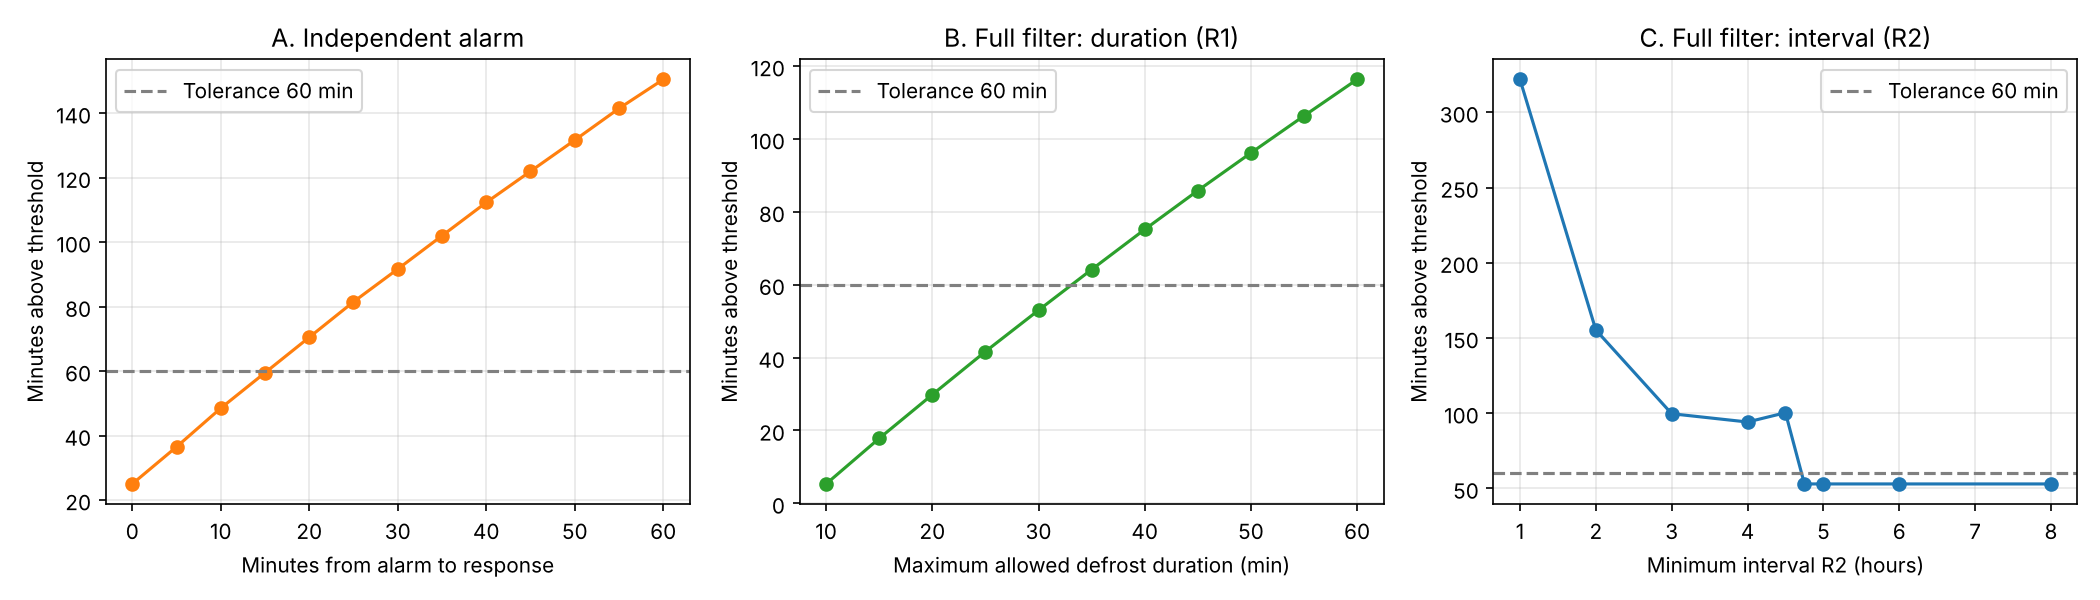
\includegraphics[width=\linewidth]{sensitivity.png}
  \caption{Minutes above the threshold as a function of the time from alarm to response (left), of the maximum allowed defrost duration (centre) and of the minimum interval between defrosts (right).}
  \label{fig:sensitivity}
\end{figure}

\subsection{Closed form versus simulation, and design limits}
\label{sec:closedform}

Table~\ref{tab:closedform} compares the closed-form expressions with the simulation, starting from $T_0 = -17.15$\degC, the cabinet temperature at 02:00.
For every defrost duration $d$ the minutes above the threshold agree within 0.1 minutes.
In the automatic-protection case the simulation gives 25.0 minutes against 24.8, because on its 10\,s grid it detects the threshold crossing at 8.0 rather than 7.9 minutes, so the defrost lasts 18.0 rather than 17.9 minutes.
The closed form also gives the two limits that the simulation could only bracket: the maximum admissible defrost duration is 33.1 minutes, between the 30 minutes that meet the criterion and the 35 that exceed it, and the maximum alarm response time is $33.1 - 7.9 - 10 = 15.2$ minutes, between 15 and 20.

\begin{table}[ht]
  \caption{Closed-form results against the simulation (full filter for $M(d)$).}
  \label{tab:closedform}
  \begin{tabular}{@{}lrr@{}}
    \toprule
    Quantity & Closed form & Simulation \\
    \midrule
    Time to cross $-15$\degC, $t_1$ & 7.9 min & 8 min \\
    Minutes above threshold, $M(20)$ & 29.9 & 29.8 \\
    Minutes above threshold, $M(30)$ & 53.1 & 53.0 \\
    Minutes above threshold, $M(35)$ & 64.3 & 64.2 \\
    Minutes above threshold, $M(40)$ & 75.2 & 75.2 \\
    Automatic protection, $M(t_1 + 10)$ & 24.8 & 25.0 \\
    Maximum admissible defrost duration, $d_{\max}$ & 33.1 min & between 30 and 35 min \\
    Maximum alarm response time, $r_{\max}$ & 15.2 min & between 15 and 20 min \\
    \bottomrule
  \end{tabular}
\end{table}

The same expressions give the limits for other cabinets (Table~\ref{tab:limits}).
For each variation of $UA$ or $P_s$, $T_0$ is recomputed from the normal night, so every row uses consistent initial conditions; the closed-form $M(30)$ agrees with the simulated full filter within 0.2 minutes in every row.
The maximum admissible defrost duration ranges from 24.6 to 53.4 minutes and the maximum alarm response time from 5.4 to 24.4 minutes.
Rows with $d_{\max} < 30$ are exactly those where the 30-minute filter exceeds the criterion in Table~\ref{tab:sensitivity}, and $r_{\max}$ stays positive in every row, consistent with the automatic protection meeting the criterion throughout.

\begin{table}[ht]
  \caption{Design limits from the closed form for different cabinets. $T_0$ is the temperature at 02:00 in the normal night, $t_1$ the time to cross $-15$\degC.}
  \label{tab:limits}
  \begin{tabular}{@{}lrrrr@{}}
    \toprule
    Cabinet & $T_0$ (\textdegree{}C) & $t_1$ (min) & $d_{\max}$ (min) & $r_{\max}$ (min) \\
    \midrule
    $UA \times 0.5$ & $-18.75$ & 19.0 & 53.4 & 24.4 \\
    $UA \times 0.75$ & $-17.10$ & 9.0 & 38.8 & 19.8 \\
    Base cabinet & $-17.15$ & 7.9 & 33.1 & 15.2 \\
    $UA \times 1.25$ & $-17.27$ & 7.3 & 27.7 & 10.4 \\
    $UA \times 1.5$ & $-18.25$ & 9.3 & 24.6 & 5.4 \\
    $P_s \times 0.5$ & $-17.15$ & 10.1 & 39.1 & 19.0 \\
    $P_s \times 0.75$ & $-17.15$ & 8.9 & 35.8 & 16.9 \\
    $P_s \times 1.5$ & $-17.15$ & 6.5 & 28.8 & 12.3 \\
    $P_s \times 2$ & $-17.15$ & 5.5 & 25.5 & 10.0 \\
    \bottomrule
  \end{tabular}
\end{table}

The practical consequence is that the limits of the defences should be computed for each cabinet from its parameters, which the closed form makes possible without simulation, rather than copied from one installation to another.

%% ===========================================================================
\section{Countermeasures for operators and maintenance companies}
\label{sec:countermeasures}

Table~\ref{tab:countermeasures} lists the countermeasures in order of effectiveness in our results.
The first three are evaluated in this work; the last two are not, and are given as good practice.

\begin{table}[ht]
  \caption{Countermeasures and their basis.}
  \label{tab:countermeasures}
  \begin{tabular}{@{}p{0.42\linewidth}p{0.24\linewidth}p{0.26\linewidth}@{}}
    \toprule
    Countermeasure & Where & Basis \\
    \midrule
    Local limits on defrost commands: maximum duration, computed for the cabinet, \emph{and} minimum interval preventing further remote defrosts before local takeover & Separate device in the store, or a local controller function that cannot be reconfigured remotely & Scenario 2, Tables~\ref{tab:sensitivity} and~\ref{tab:limits} \\
    Independent protection with automatic response (temperature band limiter): a separate, non-networked device that stops the defrost above a temperature limit & In the store, on a separate channel & Scenario 4; break-even condition~\eqref{eq:breakeven} \\
    Separation of access: credentials and nodes per store or per small group & Remote management & Table~\ref{tab:blast} \\
    No direct internet exposure, protected remote access, review of maintenance providers and credentials, update or replacement of unsupported devices & Network and supplier contracts & Not evaluated; ACN bulletin~\cite{cyber360acn2026} \\
    Emergency plan: manual operation and spare refrigerated vehicles & Organisation & Not evaluated \\
    \bottomrule
  \end{tabular}
\end{table}

\paragraph{When does an in-store protection pay for itself?}
Let $c$ be the yearly cost of a protection per store, including its purchase spread over its lifetime, installation and maintenance; $p$ the yearly probability that a successful attack reaches the store, which in a centralised architecture is the probability that the shared node is compromised, since one compromise then reaches every store; and $\Delta L$ the loss per store that the protection avoids.
The protection is worth adopting when the expected yearly loss it avoids exceeds its cost, $p\,\Delta L > c$, that is when
\begin{equation}
  p > p^{*} = \frac{c}{\Delta L}.
  \label{eq:breakeven}
\end{equation}
In scenarios 2 and 4 the protection avoids the whole loss, so $\Delta L = L = $ \texteuro{}30{,}000: a protection costing \texteuro{}100 per store per year pays for itself if $p > 0.33\%$ per year, and one costing \texteuro{}300 if $p > 1\%$; these costs are examples, not market prices.
A protection that only reduced the damage would enter the same condition with a smaller $\Delta L$.
The condition does not require an estimate of $p$, which is not known: it turns the decision into whether an operator considers a successful attack more likely than $p^*$.
It is a preliminary break-even assessment, not a full cost-benefit analysis: it neglects indirect costs such as unnecessary trips, temporary interruptions of refrigeration and failures of the protection itself.

Three operational indications follow from the results.
\begin{itemize}
  \item \textbf{Defences belong in the store.} A filter installed on the central node is bypassed by whoever controls that node.
  \item \textbf{Rules must be combined and sized.} A duration limit without a minimum interval is bypassed by repeating the command, the interval must prevent further remote defrosts before staff take over, and the duration limit must be computed for each cabinet (Table~\ref{tab:limits}).
  \item \textbf{An alarm that calls a person is a safety net, not a protection.} A response within 15 minutes is hard to guarantee at night; the independent protection should therefore act on its own.
\end{itemize}

For an operator in Campania, the first step is a question to its maintenance company: how many stores can be commanded from the same remote access?
The answer says in which row of Table~\ref{tab:blast} the operator sits.

%% ===========================================================================
\section{Limitations}
\label{sec:limitations}

The results should be read as the demonstration of a mechanism, not as measurements of real installations.
\begin{itemize}
  \item \textbf{Hypothetical chain.} How centralised remote management of supermarkets in Campania is remains unknown. The blast-radius result is conditional: it holds for operators whose nodes reach several stores.
  \item \textbf{Illustrative, lumped model.} The model is not calibrated on a real cabinet and lumps structure, air and products into one temperature: the air warms faster and the core of the products more slowly. Latent heat is neglected, which matters only near and above 0\degC. The code is verified against the closed-form solutions, but the model is not validated against measurements. The closed form assumes constant inputs within each phase and a known starting temperature, which depends on the thermostat phase.
  \item \textbf{Measured versus modelled temperature.} The independent sensor measures a local temperature, while the model uses a lumped one, and temperatures inside a cabinet vary with position~\cite{evans2007cabinets}. The simulation assumes that the two coincide; the relation between them, and therefore the alarm threshold, must be calibrated on a real cabinet.
  \item \textbf{Cabinet parameters.} The results of the filter depend on $UA$ and $P_s$ (Tables~\ref{tab:sensitivity} and~\ref{tab:limits}); the values used are illustrative, not taken from a specific cabinet.
  \item \textbf{Loss criterion.} The $-15$\degC{} threshold comes from Directive 89/108/EEC but refers to product temperature; the 60-minute tolerance is a convention of this study.
  \item \textbf{Simplified scenario.} One cabinet per store, identical stores, staff always arriving at 07:00.
  \item \textbf{Narrow threat model.} One compromised node and one command type, the defrost. Real cases also included setpoint changes~\cite{cyber360cases2026}, which a filter should bound in the same way. The in-store defences are assumed not to be remotely reconfigurable.
  \item \textbf{Cost analysis.} The protection costs are examples, and the break-even condition is a preliminary assessment: unnecessary trips, interruptions of refrigeration and failures of the protection are neglected.
  \item \textbf{Conceptual protection.} The band limiter is described at the level of a conceptual architecture and evaluated only in the model; it has not been built or tested.
  \item \textbf{Normal operation.} The rules must be compatible with the cabinet's normal defrost schedule; R2 need not span all the hours without staff, only prevent another remote command from being accepted before local takeover; if even that interval is not compatible, a different rule would be needed, such as a cap on cumulative defrost time.
\end{itemize}

%% ===========================================================================
\section{Conclusions and future work}
\label{sec:conclusions}

To \textbf{RQ1}, this work answers that the remote-management architecture determines how many stores fail together: with one compromised node, 20, 8 or 1 store in the chain studied.
To \textbf{RQ2}, it answers that a local filter with two simple rules, a maximum duration and a minimum interval sized according to the command cadence and the time of local takeover, keeps every store reached within the loss criterion even when the central node is compromised.
An alarm that requires a person to intervene lowers the temperature peak but does not keep the cabinet within the criterion; an independent protection with an automatic response does.
The state-space formulation turns these results into design limits, a maximum defrost duration of about 33 minutes and a maximum alarm response time of about 15 minutes for the base cabinet, and shows that these limits change with the cabinet's parameters and must be computed for each cabinet; the break-even condition gives operators a simple test of whether a protection is worth its cost.

The two answers are complementary rather than alternative: reducing the blast radius bounds how many stores an attacker reaches, and in-store limits bound what happens in each store reached.
For operators and maintenance companies this is a message of defence in depth: reduce the blast radius of the nodes and, at the same time, place inside each store limits that a remote attacker cannot remove.

Future work, in order of usefulness:
\begin{enumerate}
  \item collect from installers and maintenance companies in Campania how many stores depend on the same remote access;
  \item calibrate the model on data sheets or measurements from real cabinets, with separate air and product temperatures and latent heat, and calibrate the relation between the temperature measured by an independent sensor and the state of the goods;
  \item build and test a low-cost, non-networked temperature band limiter with a time limit, and estimate its real cost to apply the break-even condition;
  \item extend the threat model to setpoint changes and to several compromised nodes;
  \item study in-store verification of signed commands, to require two-person approval for commands sent to several stores.
\end{enumerate}

%% ===========================================================================
\section*{Ethics, data and code availability}

This work is entirely simulation-based: no real system was analysed, scanned or contacted.
No stores or vendors in Campania are named, and no intrusion technique is described.
The code (Python scripts depending only on matplotlib), the figures and the outputs reported in this paper are available at \url{https://github.com/lightskinF/refrigeration-blast-radius}; \texttt{python run\_all.py} reproduces every table and figure.

\section*{Declaration on Generative AI}

During the preparation of this work, the author used large language models (LLMs) for three purposes: a more rigorous formatting of the mathematical formulas, the generation of the figures in the paper, and assistance in writing the Python simulation code.
The author re-ran and checked the generated code and its results, and takes full responsibility for the publication's content.

\bibliography{references}

\end{document}
